	
\documentclass[preprint,12pt]{elsarticle}

\usepackage[spanish]{babel}
\usepackage{amssymb}
\usepackage{graphicx}
\usepackage{lineno}
\usepackage[utf8]{inputenc}
\usepackage{url}
\usepackage{natbib}

\begin{document}
	
	\begin{frontmatter}

		\title{\huge LAS NUEVAS CARACTERISTICAS DEL ESTANDAR ISO/IEC 9075:2008}
		
		\author{Huichi Contreras, Franklin Carlos               (2016054948)}
		
		\address{Tacna, Perú}
		
		\begin{abstract}
			%% Text of abstract
The ISO / IEC 9075 defines the structure and functions that we can use in the SQL-oriented database language where the structure of the Query language is described, in order to be able to make SQL statements and that are subsequently carried out successfully being these independent to the previously established or recently established SQL statements. That is why the need to improve and renew has made that from time to time new features are established in the SQL database query language, which is why this article will detail the new features that ISO / IEC 9075: 2008 brought us.
		\end{abstract}
\end{frontmatter}
%%
	%% Start line numbering here if you want
	%%
	%\linenumbers
	
	%% main text
	\section{Resumen}

El ISO / IEC 9075 nos define la estructura y funciones que podemos utilizar en el lenguaje SQL orientado a base de datos donde se describe la estructura del lenguaje Query, con el fin de poder hacer declaraciones SQL y que sean posteriormente realizadas con éxito siendo estos independientes a las declaraciones SQL anteriormente establecidas o recientemente establecidas. Es por ello que la necesidad de mejorar y renovar han hecho que cada cierto tiempo se vayan estableciendo nuevas características al SQL database query languaje, es por ello que en este artículo se detallara las nuevas características que nos trajo el ISO / IEC 9075 : 2008.

	%%
	%% Start line numbering here if you want
	%%
	%\linenumbers
	
	%% main text
\section{Introduccion}
SQL es un lenguaje de consulta textual declarativo para bases de datos relacionales. Combina consultas, actualizaciones e instrucciones administrativas en un solo idioma el idioma SQL. Las instrucciones administrativas permiten cambiar las diferentes propiedades de una base de datos mientras se está ejecutando.

	%%
	%% Start line numbering here if you want
	%%
	%\linenumbers
	
	%% main text

\section{Marco Teorico}
	
\subsection{NUEVAS CARACTERISTICAS DEL ISO / IEC 9075:2008}	

Estas son las principales caracteristicas que se pueden encontraren la version SQL 2008 :

\begin{itemize}
\item Declaración del término MERGE este comando proporciona la capacidad de INSERT programáticamente datos si no existe o ACTUALIZAR los datos.
\item Se introdujo la nueva declaración Truncate Table.
\item La declaración de variables permite una inicialización similar a la que hacemos en C++ (Declarábamos y luego lo utilizábamos). Ahora, en lugar de escribir dos declaraciones, podemos escribir una sola declaración (Ejemplo: DECLARE @COUNT INT =100).
\begin{figure}[htb]
	\begin{center}
		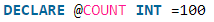
\includegraphics[width=5cm]{./IMAGENES/huichi1}
	\end{center}
\end{figure}
\item La declaración INSERT INTO ahora se puede agregar como cadena separado por una coma luego de declarar la sentencia de VALUES (Ej.: INSERT INTO Letras VALUES ((1,A), (2,B), (3,C) ) )
\begin{figure}[htb]
	\begin{center}
		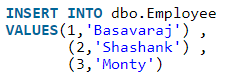
\includegraphics[width=5cm]{./IMAGENES/huichi2}
	\end{center}
\end{figure}
\item Se mejoro al momento de declarar la llave When donde se agregó como ayuda una separación por comas en una expresión que contenga la sentencia CASE.
\item Se introdujo Sparse Column que es una nueva característica más introducida en SQL SERVER 2008. Almacenar un valor nulo en una columna dispersa no ocupa espacio, pero almacenar un valor no nulo en una columna dispersa ocupa 4 bytes de espacio adicional que las columnas no dispersas de el mismo tipo de datos.
\item Se agrego nuevos tipos de datos de fecha y hora como el Date, Time, DateTime2, etc.
\item Tambien se introdujo los operadores de asignacion aritmeticos como los siguientes:
\begin{figure}[htb]
	\begin{center}
		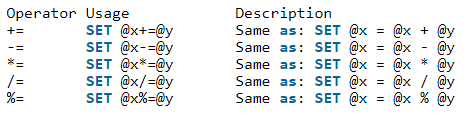
\includegraphics[width=10cm]{./IMAGENES/huichi6}
	\end{center}
\end{figure}

\end{itemize}


\section{Analisis}

Analizaremos una de las sentencias que mas causo impacto la instrucción Merge. La instrucción Merge fue lanzada en la versión 2008 con esta función podemos realizar múltiples operaciones como el INSERT, UPDATE y DELETE en los datos de la tabla de destino según sea visto en la tabla de origen y la condición que se da para llevar a cabo una unión entre ellos.
Esta característica es útil al momento de querer sincronizar datos de la tabla de destino con los datos de la tabla de origen. En versione anteriores para poder logra una sincronización, tendríamos que haber escaneado las tablas de origen y destino repetidas veces, pero con la instrucción Merge podemos lograr esto con una sola instrucción y además con una sola búsqueda en la tablas de origen y destino.

\begin{figure}[htb]
	\begin{center}
		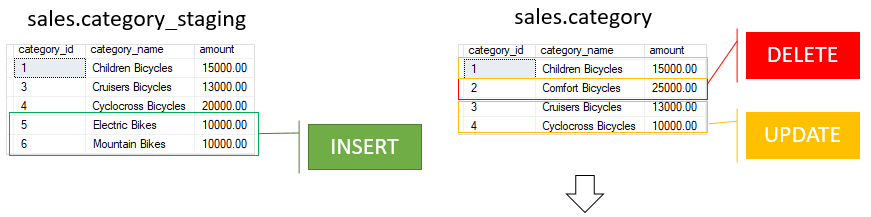
\includegraphics[width=14cm]{./IMAGENES/huichi3}
	\end{center}
\end{figure}

Por ejemplo en la imagen mostrada podemos ver que la tabla sales.category.staging y sales.category tienen los mismos campos y los mismos datos, con excepción de que tiene algunas pequeñas diferencias.

\begin{figure}[htb]
	\begin{center}
		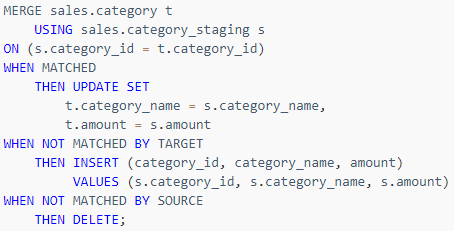
\includegraphics[width=10cm]{./IMAGENES/huichi5}
	\end{center}
\end{figure}

El código mostrado podemos ver que usamos la sentencia MERGE y vamos a alterar la tabla sales.category y usaremos la tabla sales.category.staging, estableceremos diciendo que se asemejen en su category.id ya que ambos campos lo tienen. Entonces cuando encuentren igualdades (ósea que el id de la tabla 1 sea 1 y el id de la tabla 2 sea 1) se procederá a actualizar los campos del nombre y el monto a cómo está la tabla sales.category.staging. En caso de que no encuentre igualdad en los ID entonces se insertara a los campos de sales.category los valores de la tabla sales.category.staging. Y por último como la tabla sales.category.staging no tiene el id 2 se borra quedando el resultado como es visto en la imagen.
\begin{figure}[htb]
	\begin{center}
		
\includegraphics[width=10cm]{./IMAGENES/huichi4}
	\end{center}
\end{figure}


\section{Conclusion}
La realización de la investigación acerca de las novedades que nos trajo el ISO/IEC 9075:2008 me llevaron a la conclusión de que pude aprender nuevas sentencias que fueron establecidas para resolver problemas al mantenimiento de la base de datos. Por ejemplo, el MERGE resolvía el problema que al momento de ACTUALIZAR, ELIMINAR Y AGREGAR datos de una tabla a otra vinculadas era mucho más difíciles hacerlo manualmente sin esta sentencia, o también por el lado de seguridad para poder ingresar datos exclusivos como fechas usaban los varchar esto lo arreglaron usando nuevos tipos de variables enfocadas al tiempo mejorando el filtro de entradas que se le daba a estos datos. Esto me hace pensar que todavía nos falta mucho para poder redefinir una estructura SQL finalizada o terminada, ya que cada vez que van avanzando la tecnología y los datos el manejo de la información necesita ser cada vez mejor manejada y mejor optimizada todo ello derivado a los datos que recaudemos de nuestros usuarios y para poder tener más formas de poder manejar las bases de datos. 



%%
	
	%%
	%\linenumbers
	
	%% main text

	
	\newpage
	
	\bibliographystyle{apalike} 	%ESTILO
	\bibliography{BIBLIOGRAFIA}	 
\citep{ISO1}  
\citep{ISO2}  
\citep{ISO3}  
\citep{ISO4}  
\citep{ISO5}  
	
%ARCHIVO .bib
	
	%% The Appendices part is started with the command \appendix;
	%% appendix sections are then done as normal sections
	%% \appendix
	
	%% \section{}
	%% \label{}
	
	%% References
	%%
	%% Following citation commands can be used in the body text:
	%% Usage of \cite is as follows:
	%%   \cite{key}          ==>>  [#]
	%%   \cite[chap. 2]{key} ==>>  [#, chap. 2]
	%%   \citet{key}         ==>>  Author [#]
	
	%% References with bibTeX database:
	
	
	%% Authors are advised to submit their bibtex database files. They are
	%% requested to list a bibtex style file in the manuscript if they do
	%% not want to use model1-num-names.bst.
	
	%% References without bibTeX database:
	
	% \begin{thebibliography}{00}
	
	%% \bibitem must have the following form:
	%%   \bibitem{key}...
	%%
	
	% \bibitem{}
	
	% \end{thebibliography}
	
\end{document}

%%
%% End of file `elsarticle-template-1-num.tex'.
